\section{Lab Environment}
A segmented lab environment was needed in order to accomplish the objectives of generating synthetic scanning data for comparison.
Within this chapter, the design choices and implementation details are elaborated.
Chosen virtualization platform is VMware Workstation in combination with the operating systems Ubuntu Server for scanning targets and Kali Linux for the scanning host.
A guide for installation of Kali Linux can be followed on the official Kali web page \footnote{\OrjansHref{https://www.kali.org/docs/installation/hard-disk-install/}{https://www.kali.org/docs/installation/hard-disk-install/}}.

%% ---------------------------- SOFTWARE AND OS IMPLEMENTATION ----------------------------
\subsection{Software and operating system implementation}
\label{s:LabEnv}
\begin{figure}[htbp]
\centerline{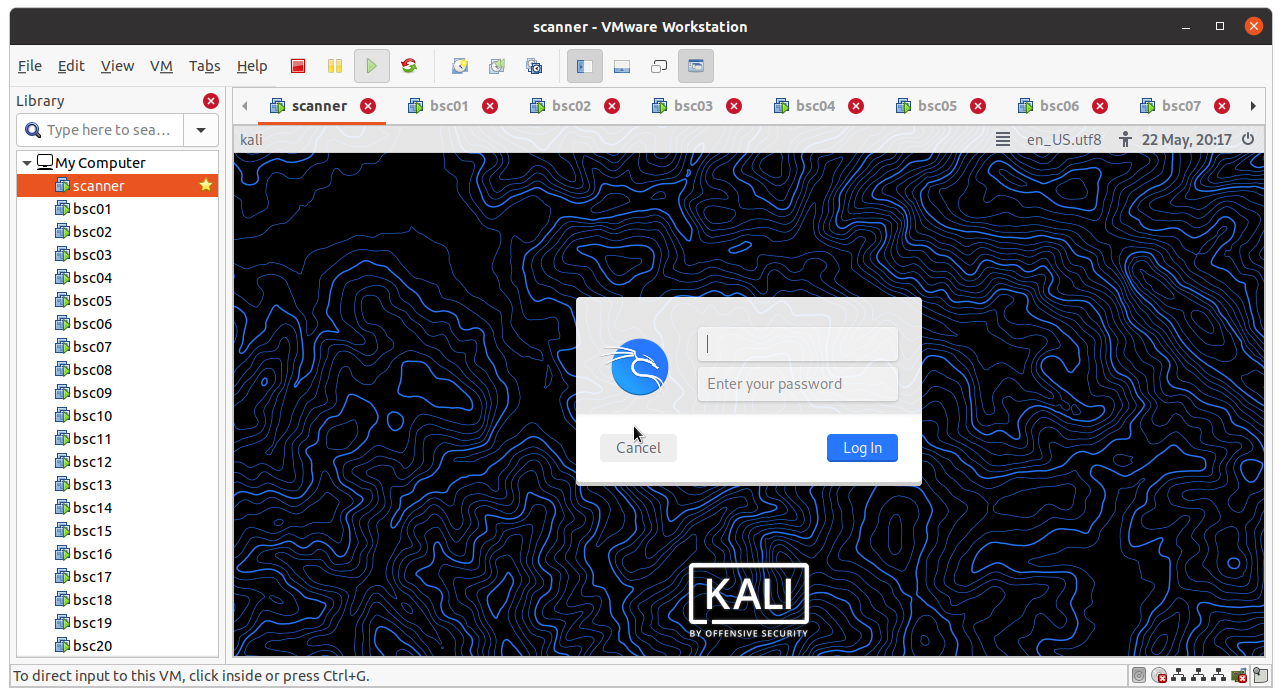
\includegraphics[scale=0.35]{images/lab/vmware-lab.png}}
\caption{Lab environment shown in VMware Workstation}
\label{fig:LabVMware}
\end{figure}

VMware Workstation 16.1 was used to set up 20 virtual hosts (referred to as workers) using Ubuntu 20.04 (Linux kernel 5.4.0-81-generic \#91) with the only target of capturing packet captures from the scanner host.
The host running the VMware Workstation is using Ubuntu Linux 20.04.4 (Linux kernel 5.13.0-35-generic \#40).
One virtual host (referred to as the scanner host) were installed with Kali Linux 2021.4 (Linux kernel 5.14.0-kali4-amd64 \#1) for conducting a various type of scans, issuing tasks to the workers, and monitoring ongoing scans.
Both these operating systems are based on Debian, which simplifies setup, configuration, and troubleshooting during the research. These operating systems are also easy to install and use without a large need for customization, which reduces the time consumption during the research as well.

%% ---------------------------- VIRTUAL NETWORK SETTINGS ----------------------------
\subsection{Virtual network settings}
\label{ss:VirtualNetworkSettings}

Two closed internal virtual networks are set up for the purpose of data generation and management.
These two networks had no connectivity to either the local network or to the internet.
The network diagram for the lab environment is shown in figure \ref{fig:LabNetwork}.

\begin{figure}[htbp]
\centerline{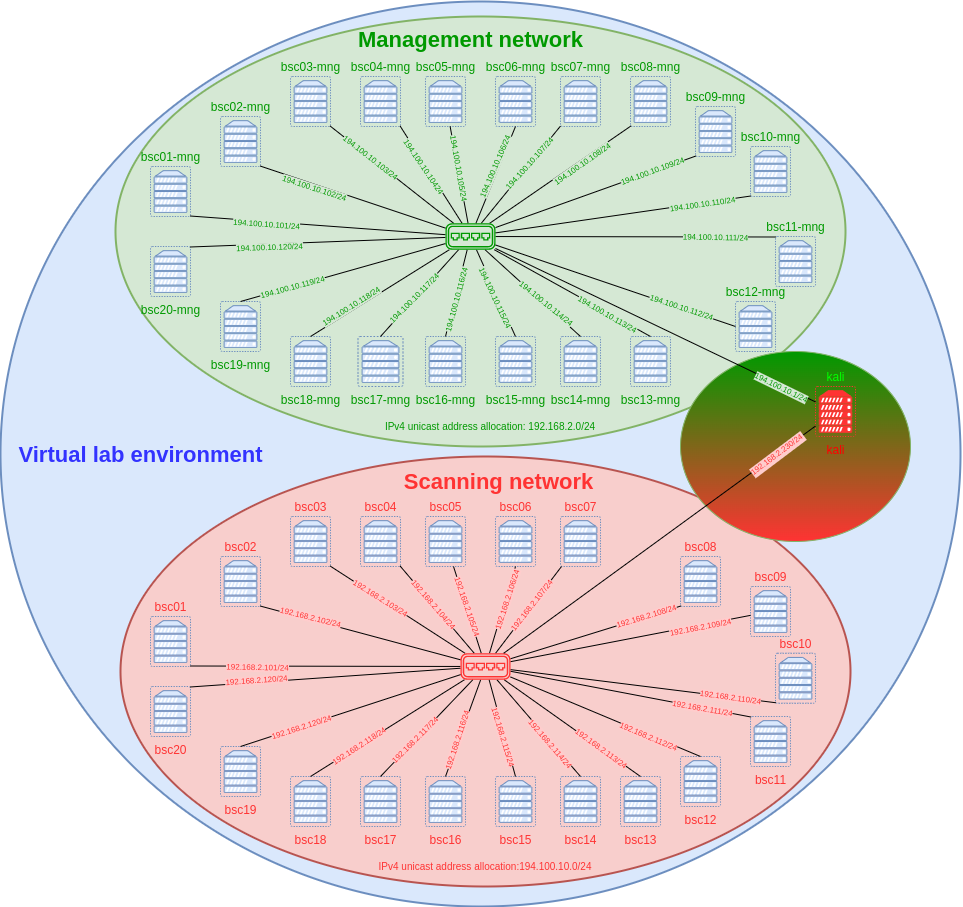
\includegraphics[scale=0.35]{images/LabNetwork.png}}
\caption{Capture of network diagram for the virtual environment.}
\label{fig:LabNetwork}
\end{figure}

The scanner host were also setup with an initial NAT network interface for retrieval of additional packets needed during the research and operating system updates primarily for the scanner host (as an initial step of the procedure while setting up the lab environment). The virtual network settings for this connection is shown in figure \ref{fig:VirtNetworkInternet}.
This connection were mainly disabled during the research to not interfer with newer versions of software during the research which could result in various results making the generated data not comparable with earlier captured data.
\begin{figure}[htbp]
\centerline{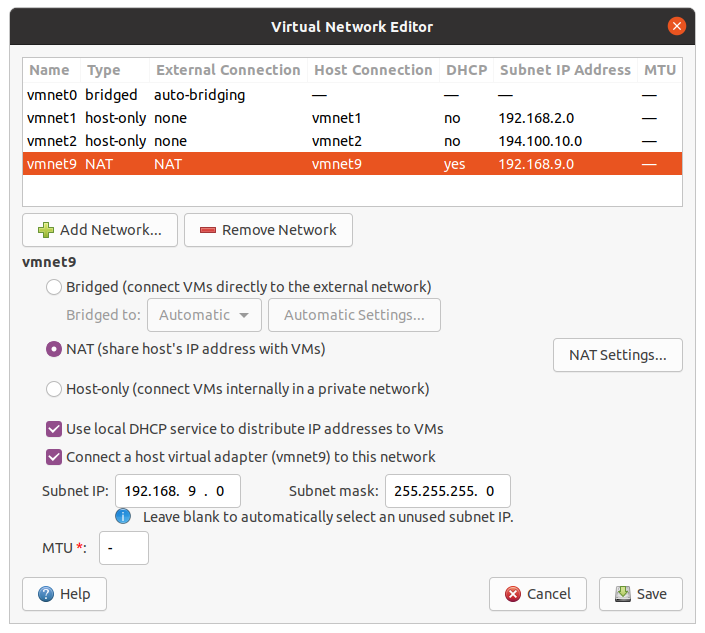
\includegraphics[scale=0.4]{images/lab/vmnet9.png}}
\caption{Virtual network settings for connectivity to internet.}
\label{fig:VirtNetworkInternet}
\end{figure}

This is for the production of raw packet captures in accordance with generating comparative data sets, which could be used for comparison between the generated synthetic data and data in the wild. Through such a comparison, these synthetic data sets could be used to classify various types of scanners and scanning types.
The chosen IPv4 unicast address block for virtual network 1 (referred to as "scanning network") is $192.168.2.0/24$, as seen in figure \ref{fig:VirtNetworkScanning}. 
Though, the address blocks $192.0.2.0/24$ is the standard for TEST-NET-1 according to RFC 5737 \autocite{rfc5737}, which describes the usage of the network during this research.
The $192.168.2.0/24$ subnet was chosen, instead of following the RFC 5737 due to other networks within the local network using this exact subnet for another experiment, to minimize confusion during the research.
Each worker host has its increment asset name where the hostname is in accordance with the last two digits in the last IP octet (e.g., $bsc01$ resolving to $192.168.2.101$). The scanning host has a higher last IP octet to ensure no confusion and IP collision regarding the static allocation for worker hosts. Within this research, the scanning host has the address $192.168.2.230$. This address allocation logic only shows flaws when the number of workers is above 99. As this is a proof of concept and the low number of workers, this is not a problem.
\begin{figure}[htbp]
\centerline{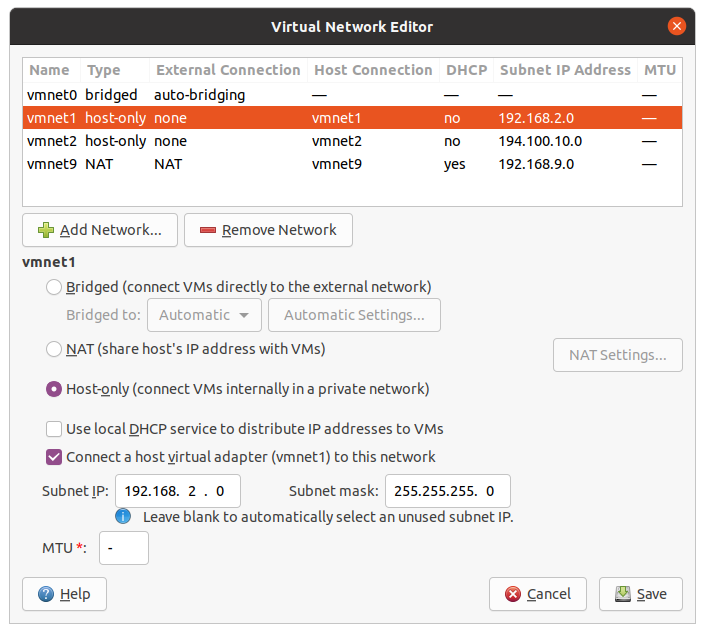
\includegraphics[scale=0.4]{images/lab/vmnet1.png}}
\caption{Virtual network settings for scanning network.}
\label{fig:VirtNetworkScanning}
\end{figure}

Secondly, another virtual network is set up for the usage of managing worker hosts in the network.
The main reason is to reduce noise traffic on the scanning network and to segment management of each worker, such as managing tasks, monitoring ongoing tasks, and retrieving raw packet capture data.
Chosen IPv4 unicast address block for the virtual network 2 (referred to as "management network") is $194.100.10.0/24$, settings shown in figure \ref{fig:VirtNetworkManagement}.
Within RFC 1466 \autocite{rfc1466} a network in the address space $194.0.0.0$ - $195.255.255.255$ is allocated for management use in Europe. The same logic for address allocation used in the scanning network is also applied to the management network, where the last IP octet represents each worker host. Both these networks are visualized in \ref{fig:LabNetwork}.
\begin{figure}[htbp]
\centerline{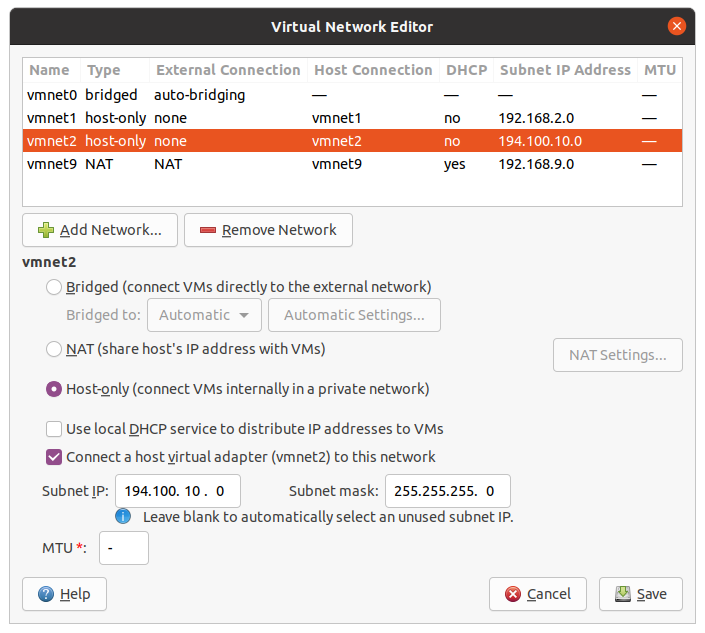
\includegraphics[scale=0.4]{images/lab/vmnet2.png}}
\caption{Virtual network settings for management network.}
\label{fig:VirtNetworkManagement}
\end{figure}
Another network characteristic is DHCP, which in both networks is disabled to ensure the logical structural setup of the network, such as static address allocation to each virtual host in accordance with a hostname.
Basing the network setup on the RFC standards reduces the possibility of collision and confusion regarding usage of the networks \autocite{rfc1466,rfc5737}.

%% ---------------------------- /VIRTUAL NETWORK SETTINGS ----------------------------